\block{\begin{blockbody}\section{Generating synthetic 3D embryos}
    \tfont
    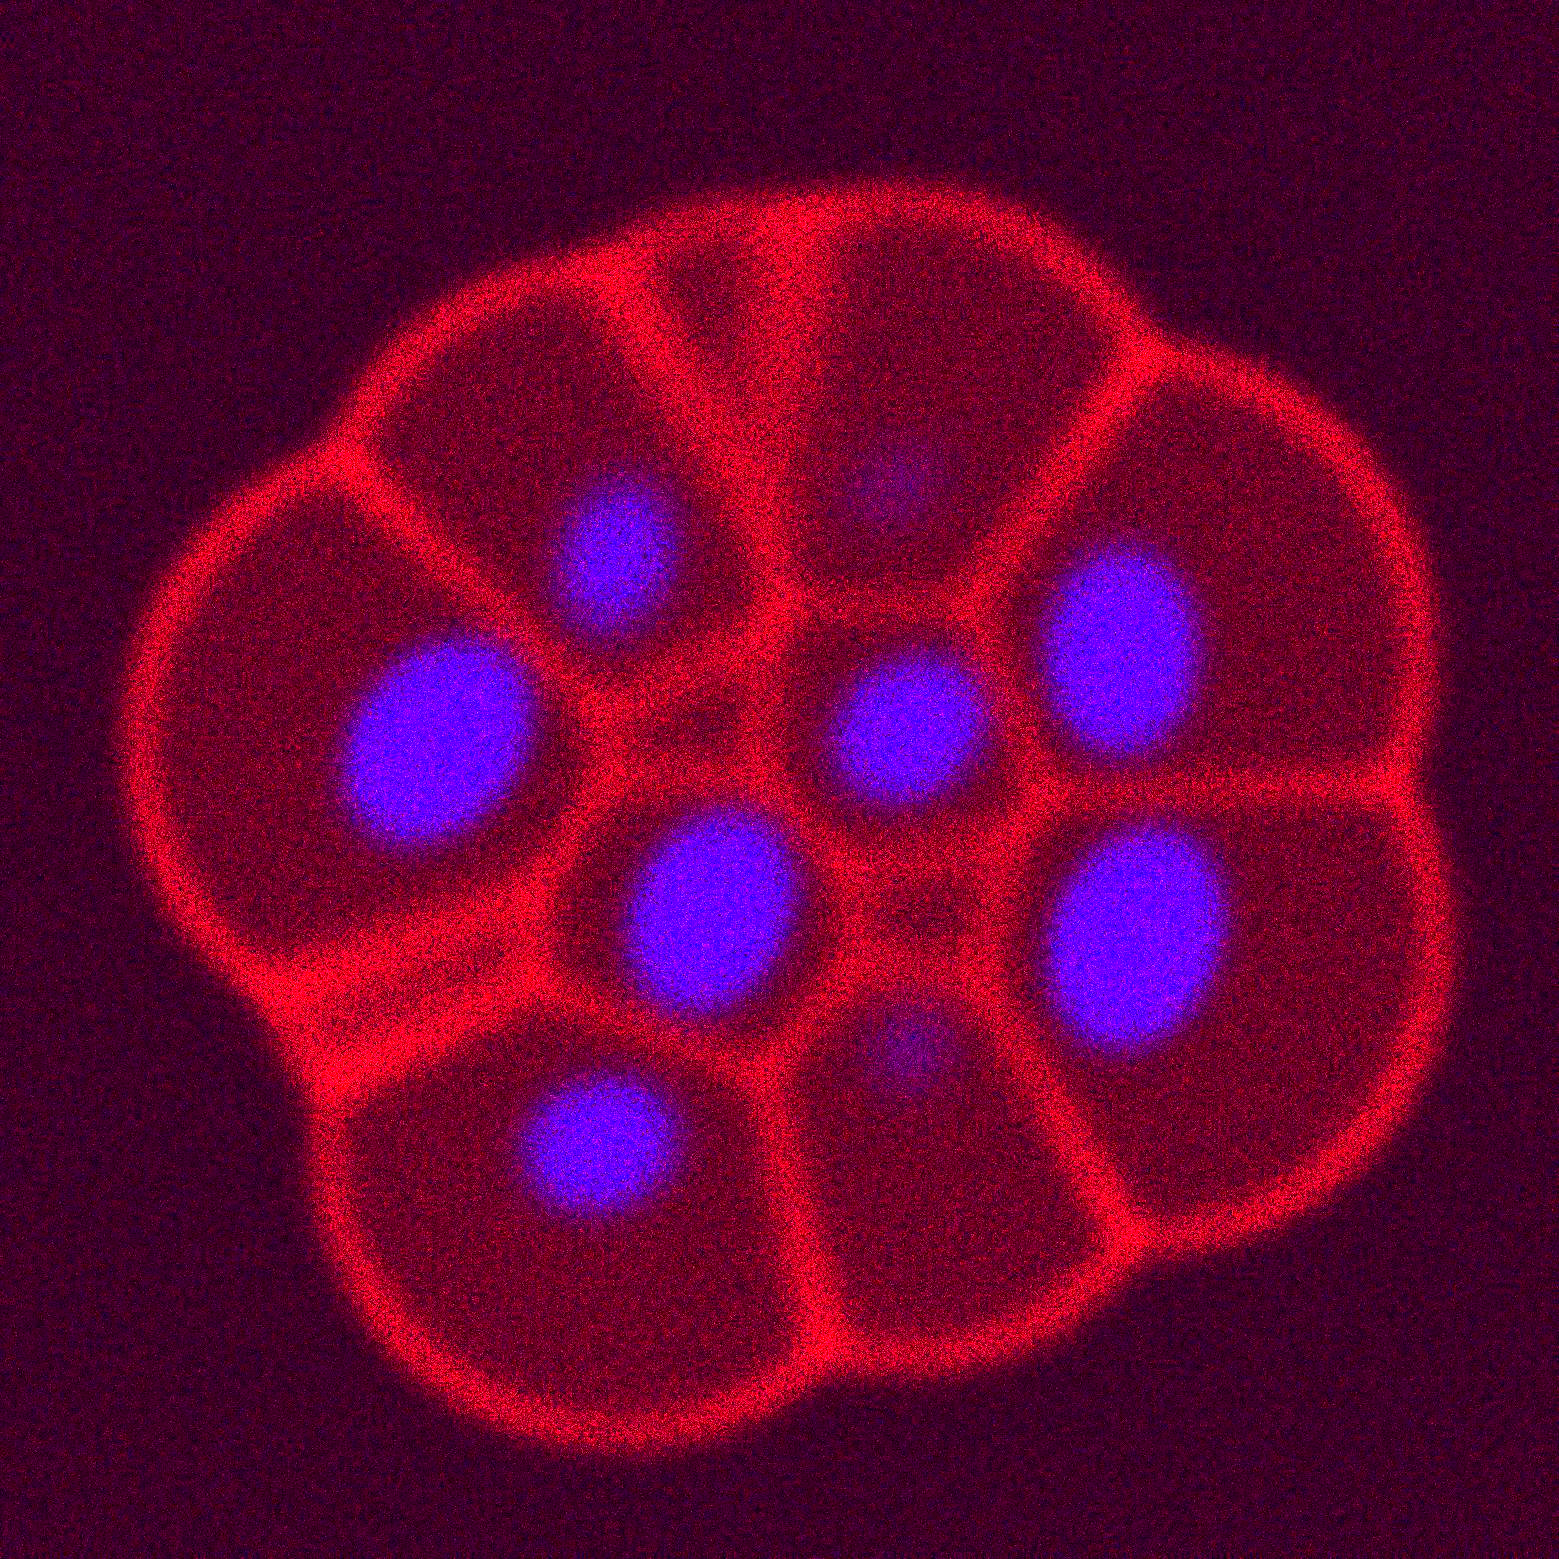
\includegraphics[width=0.49\textwidth]{images/SimEmbryo.png} \hfill
    \includegraphics[width=0.49\textwidth]{images/GroundTruth.png} \par
    \vs\vs
        Using a modification of a previously-described method \cite{Rajasekaran2016}, we generated synthetic embryo data to act as ground truths with which to test the accuracy of GIANI. Three populations were generated, each exhibiting a different signal-to-noise ratio (SNR). There were 10 embryos in each population and the number of cells in each embryo ranged from 15 to 35.
\end{blockbody}}